\begin{multicols*}{2}
\section*{12. Thermal Radiation Fundamentals}
\subsection*{9.1. General Procedure}
Most questions will ask for irradiation given some geometry and temperatures.
\begin{enumerate}
    \item Determine absorptivity $\alpha$, reflectivity $\rho$, and transmissivity $\tau$ using the geometry and material properties. 
    Note that if two of these are known, the third can be found using $\alpha + \rho + \tau = 1$.
    \item Use solid angle $\omega$, irradiation $G$, and intensity $I$ to find whatever is asked for
\end{enumerate}
\subsection*{9.2. Variable Definitions}
\begin{itemize}
    \item $\omega$: Solid angle
    \item $G$: Irradiation
    \item $I$: Intensity
    \item $J$: Radiosity
    \item $\dot{Q}$: Heat transfer rate
    \item $\alpha$: Absorptivity
    \item $\rho$: Reflectivity
    \item $\tau$: Transmissivity
    \item $\epsilon$: Emissivity
    \item $\sigma$: Stefan-Boltzmann constant
\end{itemize}

\subsection*{9.3. Formulas}
For $A \ll r^2$ (small area, far away from surface),
\begin{align*}
    \omega_{2-1} &:= \frac{A_2 \cos\theta_2}{r^2}\\
    J_1 &:= \pi I_{1, e+r} = \pi(E_b + G_{\text{ref}}) = \pi(\epsilon\sigma T_{1}^4  + \rho G_{1}) \\ 
    \dot{Q}_{1-2} &:= I_1 (A_1 \cos\theta_1) \omega_{2-1} \\
    G_2 &:= \frac{\dot{Q}_{1-2}}{A_2} 
\end{align*}
Combining the above equations into $G_2$,
\begin{align*}
    G_2 &= \frac{(\epsilon\sigma T_{1}^4  + \rho G_{\text{1}})A_1 \cos\theta_1 \cos\theta_2}{\pi r^2} 
\end{align*}
Since $\theta_1 = \theta_2 = \rho = 0$ and $\epsilon = 1$ for a blackbody,
\begin{align*}
    G_2 &= \frac{\sigma T_{1}^4 A_1}{\pi r^2} \\
    \implies T_{1} &= \left(\frac{G_2 \pi r^2}{\sigma A_1}\right)^{1/4}
\end{align*}

\end{multicols*}

\section*{Tables}
% \begin{table}[H]
%     \centering
%     \caption{Empirical correlations for the average Nusselt number for natural convection over surfaces 
%     (\textbf{Table 9-1 in textbook})}
%     \label{tab:sec9_natural_convection_over_surfaces}
%     \begin{tabular}{p{0.2\textwidth}p{0.1\textwidth}p{0.15\textwidth}p{0.4\textwidth}}
%         \hline
%         Geometry & Characteristic Length $L_c$ & Range & Nu \\
%         \hline
%         \multirow{2}{*}{Vertical Plate 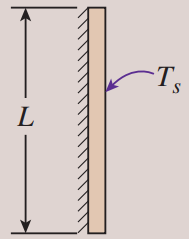
\includegraphics[width=0.1\textwidth]{Figures/Sec9 Vertical Plate.png}} 
%         & $L$ & $10^4 \leq \text{Ra}_L \leq 10^{9}$ & $\displaystyle \text{Nu} =0.59 \text{Ra}_L^{1/4}$ \\
%         & & $\displaystyle 10^{9} \leq \text{Ra}_L \leq 10^{13}$ & $\text{Nu} = 0.1 \text{Ra}_L^{1/3}$ \\
%         & & Entire range & $\displaystyle \text{Nu} = \left(0.825 + \frac{0.387 \text{Ra}_L^{1/6}}{[1 + (0.492/\text{Pr})^{9/16}]^{8/27}}\right)^2$ \\
%         & & & (complex but more accurate) \\
%         & & & \\
%         \hline
%         \multirow{2}{*}{Inclined Plate 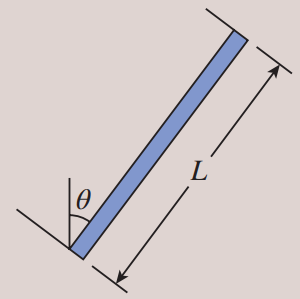
\includegraphics[width=0.1\textwidth]{Figures/Sec9 Inclined Plate.png}}
%         & $L$ & & Use vertical plate equations for the upper 
%         surface of a cold plate and the lower 
%         surface of a hot plate \\
%         & & & \\
%         & & & Replace $g$ with $g \cos\theta$ for $0 < \theta < 60^\circ$ \\
%         & & & \\
%         \hline
%         % finish later
%     \end{tabular}
% \end{table}
\begin{table}[H]
    \centering
    \caption{Empirical correlations for the average Nusselt number for natural convection over surfaces 
    (\textbf{Table 9-1 in textbook})}
    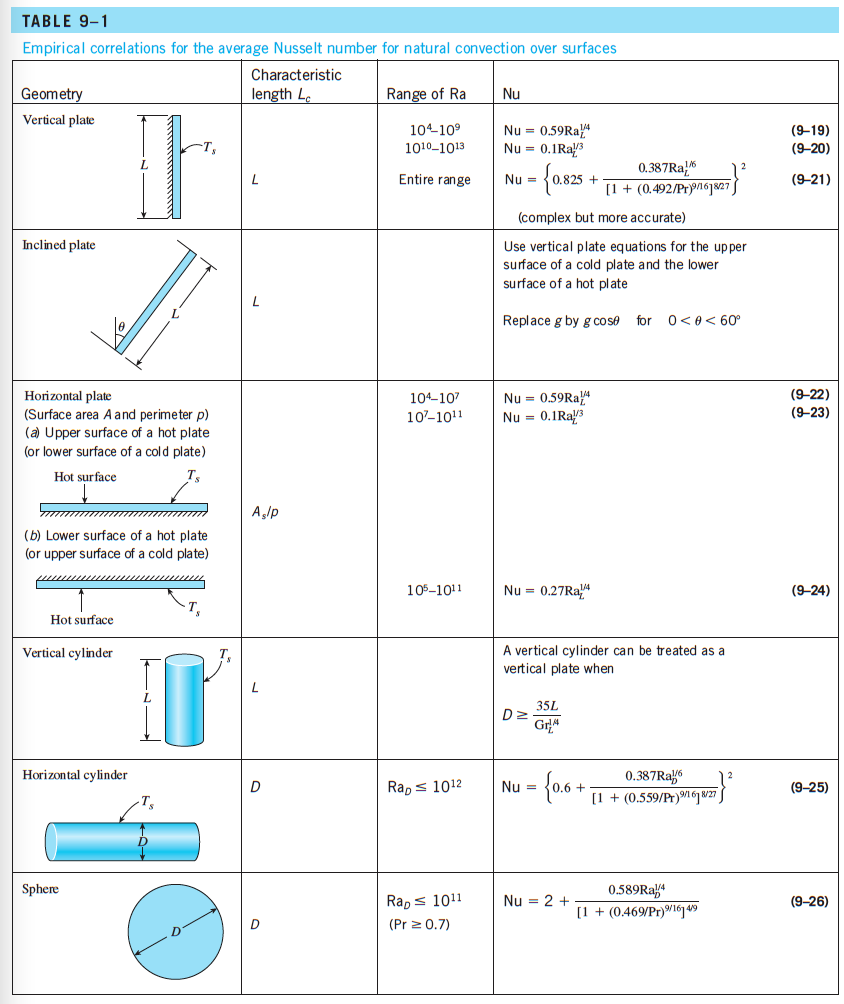
\includegraphics[width=1\textwidth]{Figures/sec9 table 9-1.png}
    \label{tab:sec9_natural_convection_over_surfaces}
\end{table}

% %     \centering
%     \caption{Nusselt number and friction factor for fully developed laminar flow in tubes of various cross sections 
%     ($D_h = 4A_c /P$, $Re = V_{\text{avg}} D_h / \nu$, and $\text{Nu} = hD_h / k$) (\textbf{Table 8-1 in textbook})}
%     \label{tab:sec8_fully_developed_laminar}
%     \begin{tabular}{ccccc}
%         \hline
%         & & \multicolumn{2}{c}{Nu} & \\
%         \cline{3-4}
%         Tube Geometry & $a/b$ or $\theta^\circ$ & $T_s = \text{constant}$ & $\dot{q}_s = \text{constant}$ & $f$ \\
%         \hline
%         \raisebox{-\totalheight}{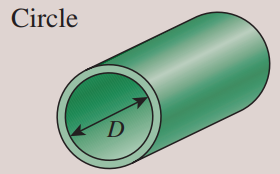
\includegraphics[width=0.15\textwidth]{Figures/Sec8 Circle Fully Laminar.png}} & --- & 4.36 & 3.66 & 64/Re \\
%         \hline
%         & \underline{$a/b$} & & & \\ 
%         \multirow{2}{*}{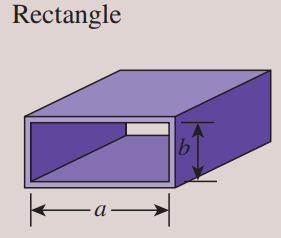
\includegraphics[width=0.15\textwidth]{Figures/Sec8 Rectangle Fully Laminar.png}} 
%         & 1 & 2.98 & 3.61 & 56.92/Re \\
%         & 2 & 3.39 & 4.12 & 62.20/Re \\
%         & 3 & 3.96 & 4.79 & 68.36/Re \\
%         & 4 & 4.44 & 5.33 & 72.92/Re \\
%         & 6 & 5.14 & 6.05 & 78.80/Re \\
%         & 8 & 5.60 & 6.49 & 82.32/Re \\
%         & $\infty$ & 7.54 & 8.24 & 96.00/Re \\
%         \hline
%         & \underline{$a/b$} & & & \\
%         \multirow{2}{*}{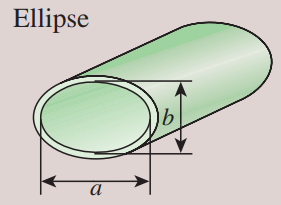
\includegraphics[width=0.15\textwidth]{Figures/Sec8 Ellipse Fully Laminar.png}}
%         & 1 & 3.66 & 4.36 & 64.00/Re \\
%         & 2 & 3.74 & 4.56 & 67.28/Re \\
%         & 4 & 3.79 & 4.88 & 72.96/Re \\
%         & 8 & 3.72 & 5.09 & 76.60/Re \\
%         & 16 & 3.65 & 5.18 & 78.16/Re \\
%         \hline
%         & \underline{$\theta^\circ$} & & & \\
%         \multirow{2}{*}{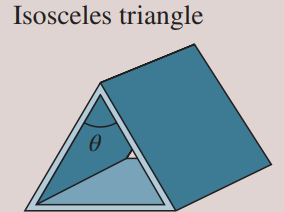
\includegraphics[width=0.15\textwidth]{Figures/Sec8 Triangle Fully Laminar.png}}
%         & 10 & 1.61 & 2.45 & 50.80/Re \\
%         & 30 & 2.26 & 2.91 & 52.28/Re \\
%         & 60 & 2.47 & 3.11 & 53.32/Re \\
%         & 90 & 2.34 & 2.98 & 52.60/Re \\
%         & 120 & 2.00 & 2.68 & 50.96/Re \\
%         \hline
%         % \raisebox{-\totalheight}{\includegraphics[width=0.15\textwidth]{Figures/Sec8 Square Fully Laminar.png}} & 1 & 3.66 & 3.11 & 64/Re \\
%     \end{tabular}